%\color{cyan} %color de texto con 70-80 % o más de avance
\section{Sensado remoto, plataformas (¿?) (Bloque 1)}
\subsection{Reservas de bosque nativo de la Selva Paranaense en la Provincia de Misiones}
El remanente en pie del bioma conocido como Bosque Atlántico o Selva Paranaense representa hoy un 5\% de la histórica extensión, que cubría desde toda la provincia de Misiones, buena parte del Paraguay y el sur de Brasil. En la provincia de Misiones está presente casi la mitad de ese remanente, existiendo varias reservas, tanto públicas como privadas. Algunas de ellas son descriptas en el presente trabajo.

\subsubsection{Reserva Biósfera Yaboty}
Para conocer de manera aproximada el tiempo que sería necesario para completar un relevamiento fotográfico aéreo territorial, tomamos como ejemplo el área de la biosfera Yaboty, cuya extensión es de 253.773 ha [1].
\begin{table}[H]
    \centering
    \begin{tabular}{|c|c|c|}
        \hline
        \textbf{Reserva} & Biósfera Yaboty &   \multirow{ 3}{*}{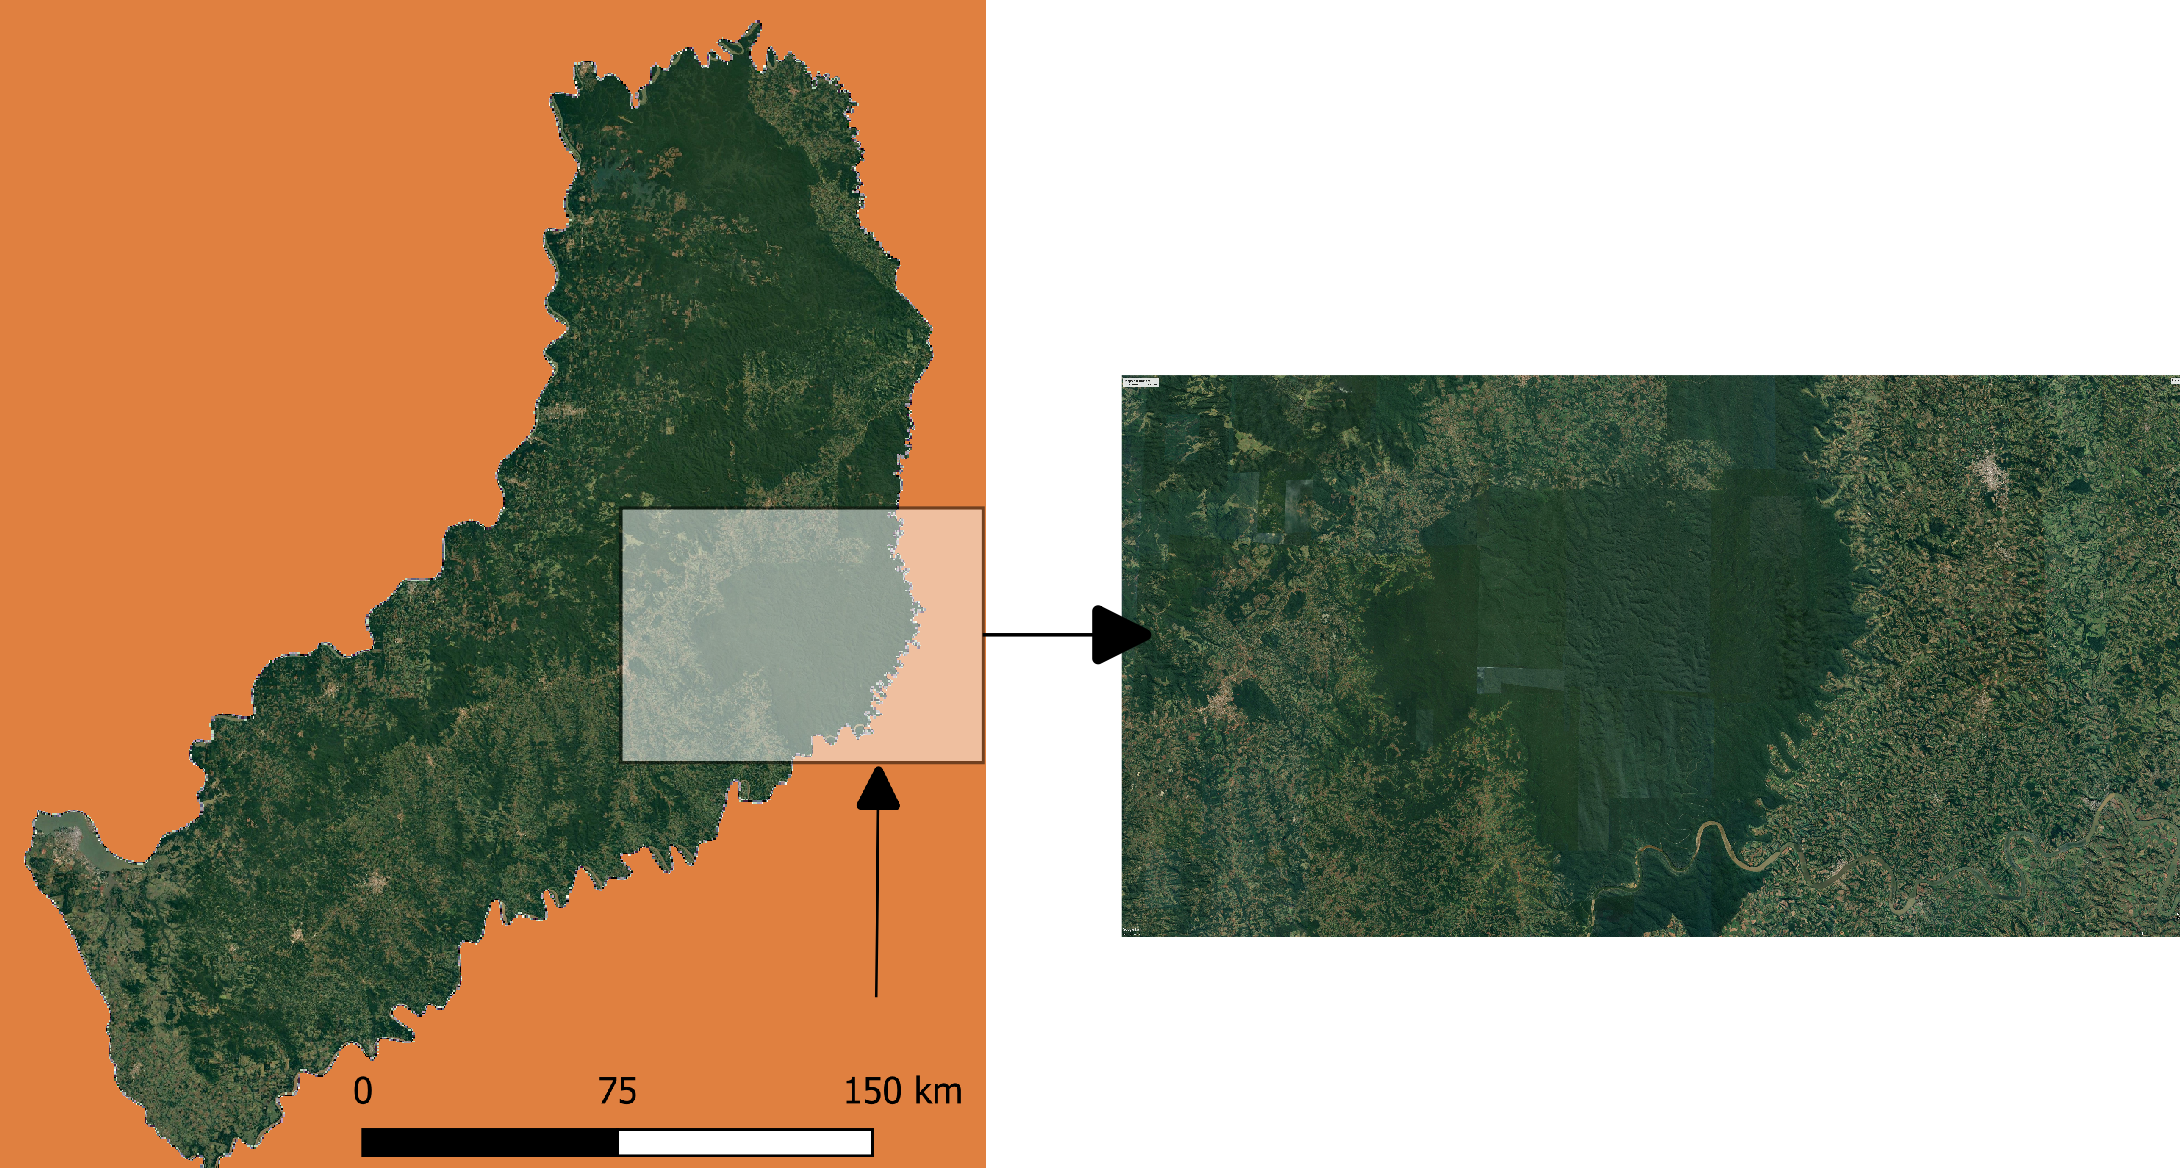
\includegraphics[width=30mm]{Imagenes/Yaboty.png}}\\ 
        \textbf{Administración} & Pública\\
        \textbf{Ubicación} & E 53° 40’, O 54° 18’, N 26° 37’ S 27° 12’ \\
        \textbf{Superficie} & 253.773 ha\\
        \hline
    \end{tabular}
    \label{Yaboty}
\end{table}
\subsubsection{Reserva San Sebastián de la Selva}
\begin{table}[H]
\centering
\begin{tabular}{|c|c|c|}
\hline
 \textbf{Reserva} & San Sebastián de la Selva &   \multirow{ 3}{*}{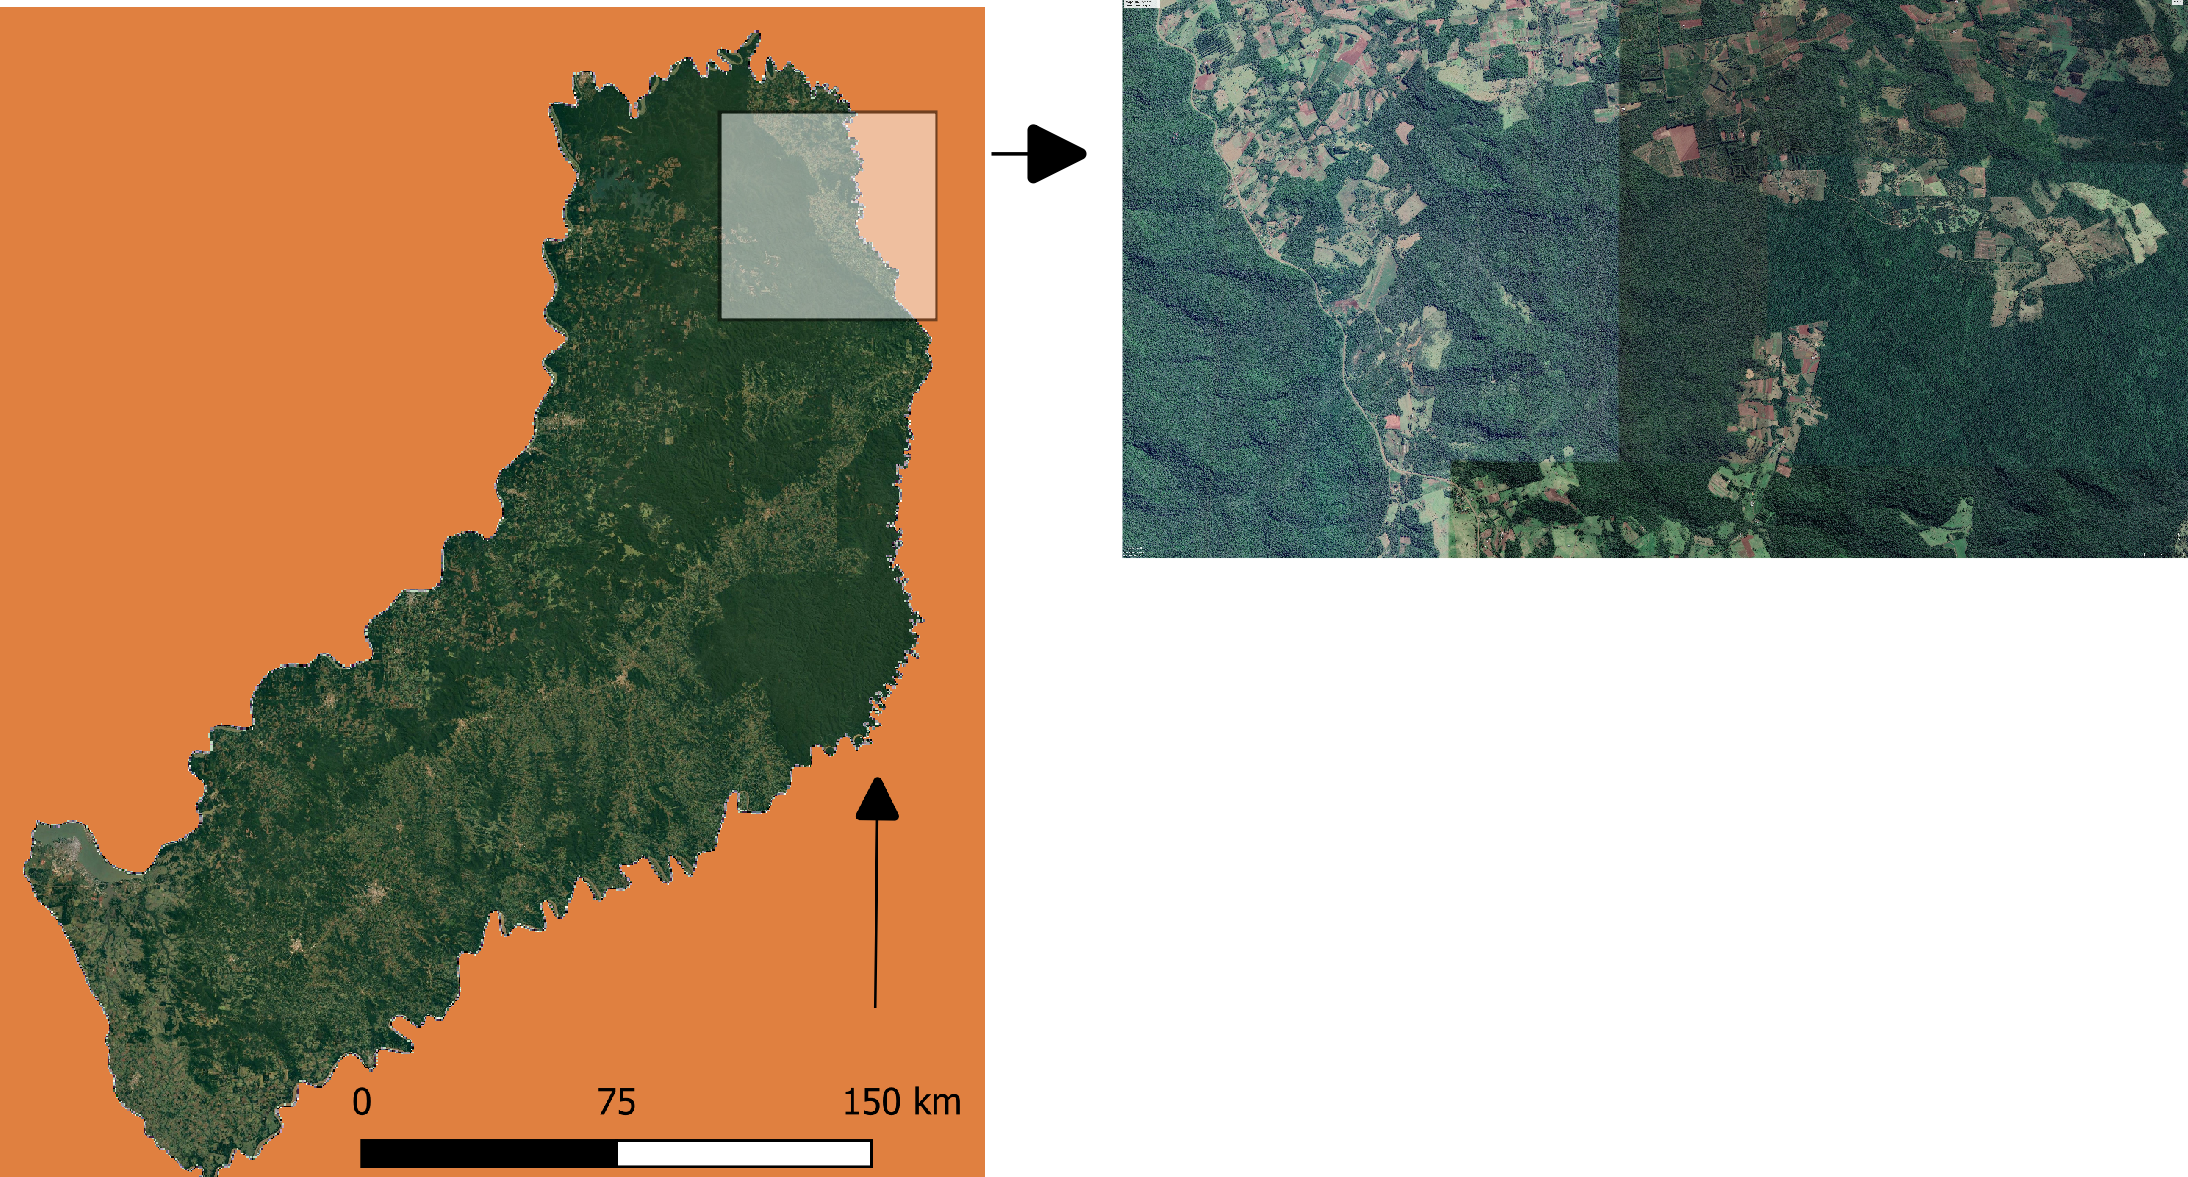
\includegraphics[width=30mm]{Imagenes/San Sebastian.png}}\\ 
\textbf{Administración} & Privada\\
        
        \textbf{Ubicación} & -25,857; -53,976 \\
         
        \textbf{Superficie} & 92 ha\\
\hline        
\end{tabular}

\label{Profundidad}
\end{table}
La reserva San Sebastián de la Selva es una reserva privada de cien hectáreas, que contiene áreas de selva virgen y de selva en restauración. Está ubicada en la localidad de Comandante Andresito, al norte de la provincia de Misiones, sobre la ruta nacional 101, entre los parques Urugua-í y Foerster. 
\subsubsection{Parque Provincial Cañadón de Profundidad}
\begin{table}[H]
\centering
\begin{tabular}{|c|c|c|}
\hline
 \textbf{Reserva} & Parque Provincial Cañadón de Profundidad &   \multirow{ 3}{*}{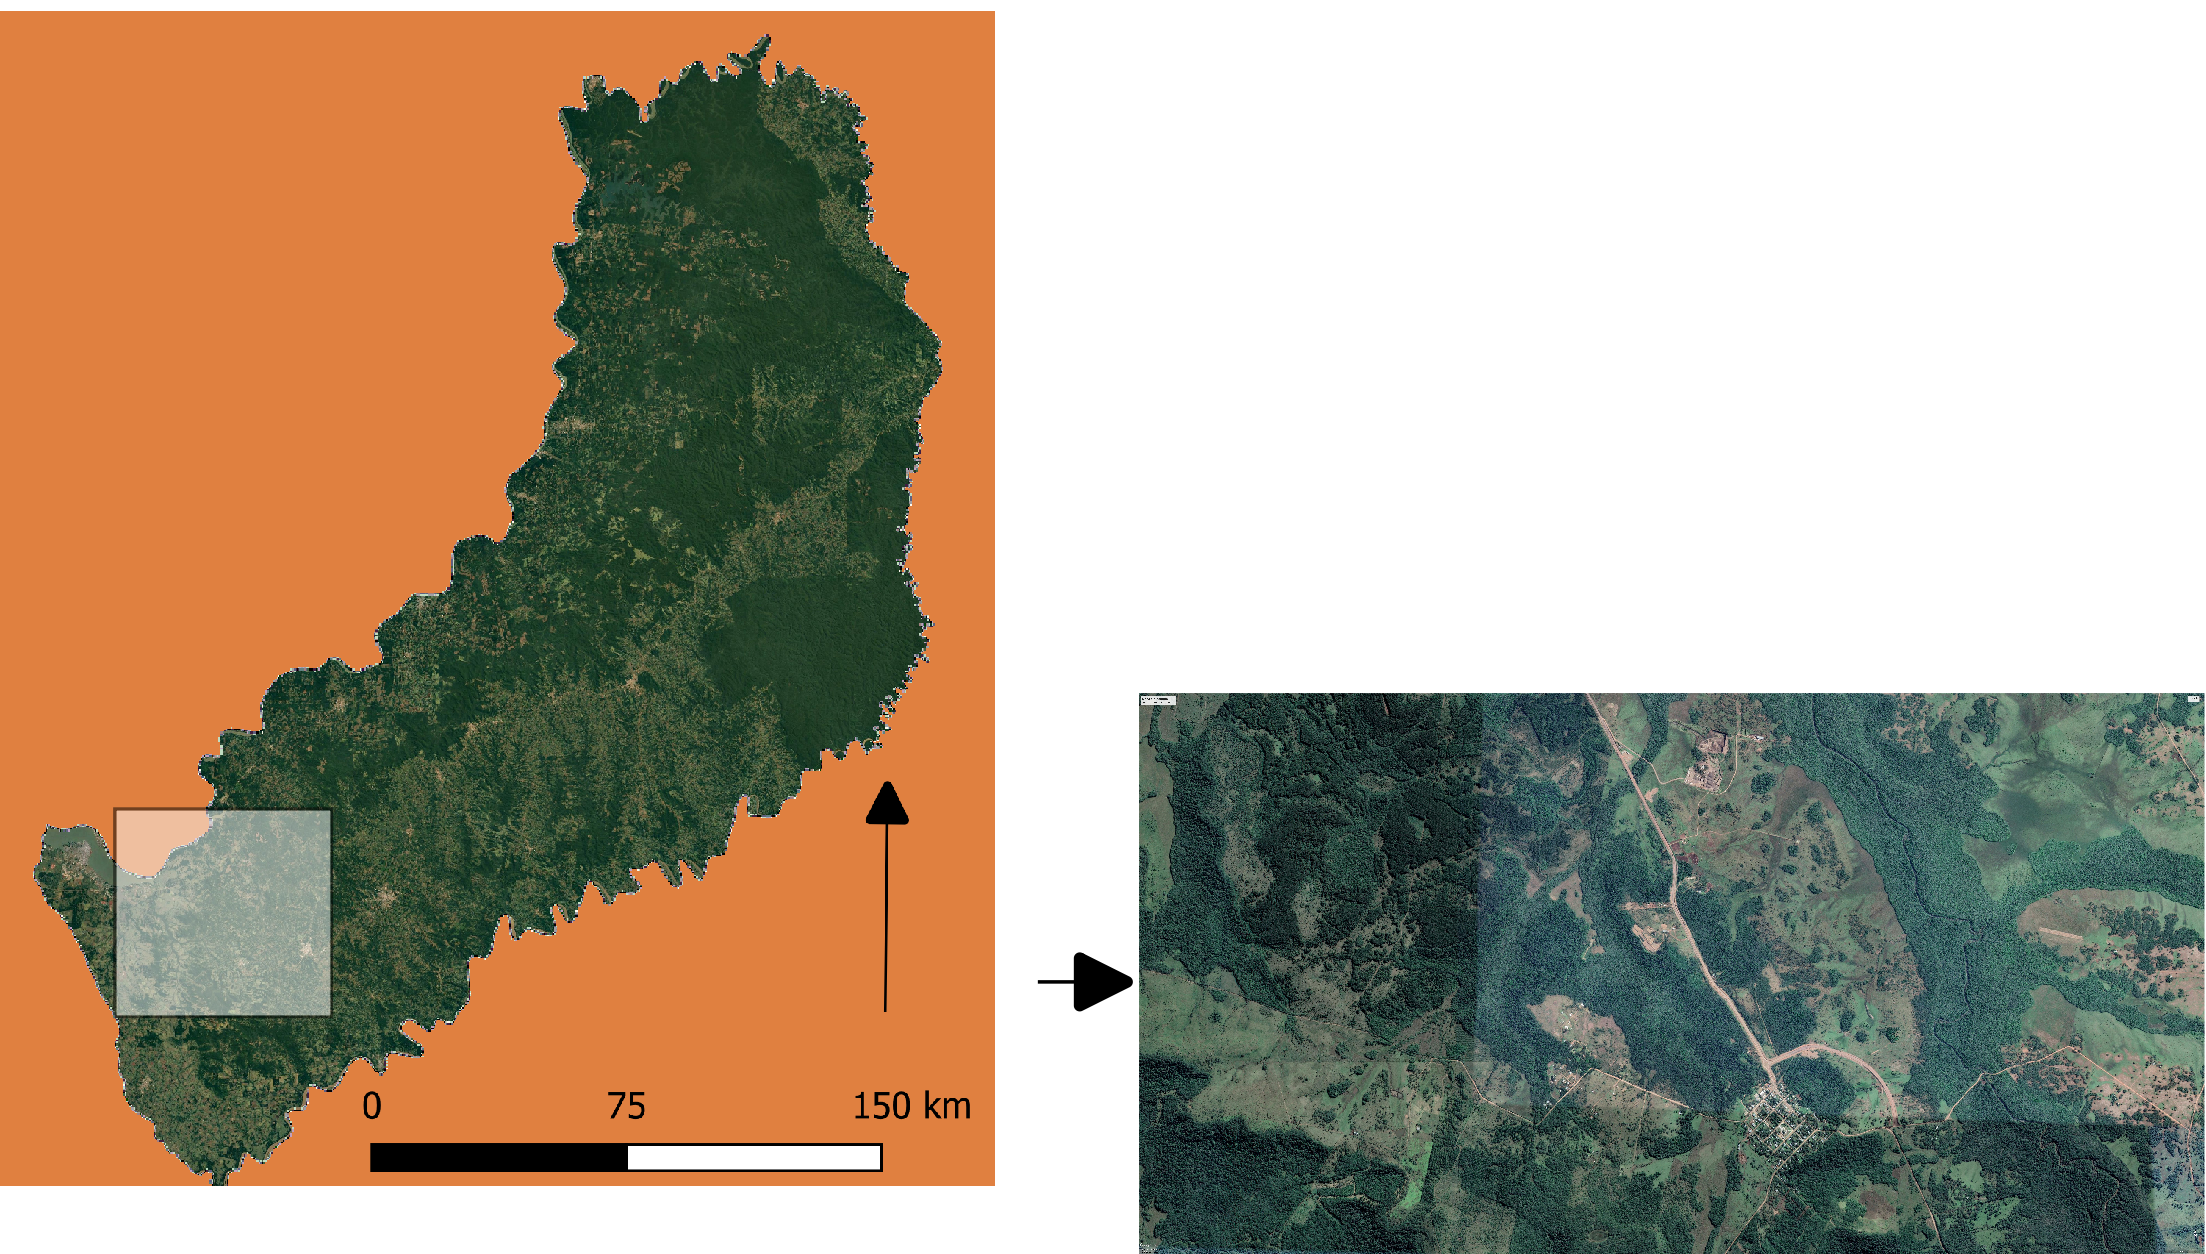
\includegraphics[width=30mm]{Imagenes/Profundidad.png}}\\ 
\textbf{Administración} & Pública\\
        
        \textbf{Ubicación} & -27,558; -55,702 \\
         
        \textbf{Superficie} & 19 ha\\
\hline        
\end{tabular}

\label{Profundidad}
\end{table}
\subsection{Requerimientos y restricciones}
\label{calculo relevamiento}
Para llevar adelante el relevamiento de las áreas forestales hay que tener en cuenta los requerimientos en el tiempo y en el equipamiento, así como las restricciones que imponen las regulaciones legales y condiciones geográficas y meteorológicas. Dependiendo de cuán grande sea el área a relevar, puede resultar más conveniente alguna de las plataformas de sensado remoto que otra. El criterio que debe ponderarse está basado en cálculos de tiempo, de costos operacionales y de disponibilidad. Para distintos escenarios, reservas grandes de miles de hectáreas de extensión o pequeñas reservas privadas de pocas decenas o centenas de hectáreas, los cálculos arrojarán resultados diferentes.
\subsubsection{Cálculo de factor de escala}
Para poder comparar entre las diferentes opciones de plataformas para captura de imágenes aeroespaciales, es necesario conocer determinados parámetros de cada una. Un parámetro es el tiempo necesario para captura de imágenes de un determinado área. El costo asociado a la operación de captura de imágenes es otro parámetro a ser tenido en cuenta. Finalmente hay otros parámetros sobre los que las opciones pueden soportarse. Uno es el porcentaje de área útil sobre área total relevada. Otro parámetro es el espacio de almacenamiento requerido.
Si se comparan imágenes obtenidas por satélites contra aquellas obtenidas por aeronaves tripuladas o VANT, resulta evidente que aquellas cubren una extensión mayor, por lo que una sola captura puede exceder en mucho la zona de interés. 
Para hallar el factor de escala $m_b$, relacionamos la altura de vuelo $H_g$ con la distancia focal
de la cámara $f$ mediante la ecuación \ref{escala} \cite{linder_digital_2016}:
 %%%%%%%%%%%%%%%%%%%%%%%%%%%%%%%%%%%%%% ECUACIÓN %%%%%%%%%%%%%%%%%%%%%%%%%%%%%%%%%%%%%%%%%%%%%%%%%%%%%%%%%
\\
\begin{equation}
	m_b=\frac{H_g}{f},\label{escala}
\end{equation}
\\
%%%%%%%%%%%%%%%%%%%%%%%%%%%%%%%%%%%%%%%%%%%%%%%%%%%%%%%%%%%%%%%%%%%%%%%%%%%%%%%%%%%%%%%%%%%%%%%%%%%%%%%%%
Para hallar cualquier distancia en la superficie real a partir de la fotografía, se aplica la relación de escala:
 %%%%%%%%%%%%%%%%%%%%%%%%%%%%%%%%%%%%%% ECUACIÓN %%%%%%%%%%%%%%%%%%%%%%%%%%%%%%%%%%%%%%%%%%%%%%%%%%%%%%%%%
\\
\begin{equation}
	S=\frac{S'H_g}{f},\label{escala1}
\end{equation}
\\
%%%%%%%%%%%%%%%%%%%%%%%%%%%%%%%%%%%%%%%%%%%%%%%%%%%%%%%%%%%%%%%%%%%%%%%%%%%%%%%%%%%%%%%%%%%%%%%%%%%%%%%%%
donde $S$ es la distancia en la superficie real, $S'$ es la distancia en la imagen.
En un relevamiento fotogramétrico, el solapamiento longitudinal suele ser de un promedio de 60\%, mientras que el solapamiento lateral suele ser de 25\% [4]. La distancia longitudinal $B$ entre dos fotografías consecutivas (línea de base) se halla en función al solapamiento longitudinal $p$, y se calcula según la ecuación (\ref{linea_de_base}).
 %%%%%%%%%%%%%%%%%%%%%%%%%%%%%%%%%%%%%% ECUACIÓN %%%%%%%%%%%%%%%%%%%%%%%%%%%%%%%%%%%%%%%%%%%%%%%%%%%%%%%%%
\\
\begin{equation}
	B=S(1-\frac{p}{100}),\label{linea_de_base}
\end{equation}
\\
%%%%%%%%%%%%%%%%%%%%%%%%%%%%%%%%%%%%%%%%%%%%%%%%%%%%%%%%%%%%%%%%%%%%%%%%%%%%%%%%%%%%%%%%%%%%%%%%%%%%%%%%%
La distancia $a$ entre dos líneas de sobrevuelo adyacentes se define por el solapamiento lateral $q$.
  %%%%%%%%%%%%%%%%%%%%%%%%%%%%%%%%%%%%%% ECUACIÓN %%%%%%%%%%%%%%%%%%%%%%%%%%%%%%%%%%%%%%%%%%%%%%%%%%%%%%%%%
\\
\begin{equation}
	a=S(1-\frac{q}{100}),\label{distancia_adyacente}
\end{equation}
\\
%%%%%%%%%%%%%%%%%%%%%%%%%%%%%%%%%%%%%%%%%%%%%%%%%%%%%%%%%%%%%%%%%%%%%%%%%%%%%%%%%%%%%%%%%%%%%%%%%%%%%%%%%
Cuando se trata de un vuelo para realizar fotografías aéreas, ya sea tripulado o no, partiendo de conocer el área de interés, sus dimensiones, es posible definir las trayectorias de vuelo. De esta forma el relevamiento fotográfico aéreo se asemeja a una especie de "barrido", con varias líneas adyacentes. A lo largo de una línea se capturan imágenes de modo que se superpongan como mínimo en un 80\% dos fotografías consecutivas. Al final de cada línea la aeronave ejecuta un giro de 180º respecto al eje nadir-cenit de modo que al finalizar el giro su proa apunte en dirección contraria a la que tenía antes de iniciar el giro. Así inicia el recorrido de una nueva línea de vuelo, la cual es paralela a la anterior, separada una distancia que garantice un solapamiento mínimo de 25\%de imágenes en líneas de vuelo adyacentes. A partir de todo ello puede establecerse la cuenta de imágenes totales que cubran toda el área, así como el tiempo necesario para llevarlo a cabo. De esto también se obtiene el espacio de almacenamiento en memoria requerido.
La cantidad de imágenes por línea de vuelo $I_lv$ se puede conocer dada la longitud de la línea de vuelo $L_v$ y la línea de base $B$, mediante la ecuación (\ref{cantidad_imagenes}):
  %%%%%%%%%%%%%%%%%%%%%%%%%%%%%%%%%%%%%% ECUACIÓN %%%%%%%%%%%%%%%%%%%%%%%%%%%%%%%%%%%%%%%%%%%%%%%%%%%%%%%%%
\\
\begin{equation}
	I_{lv}=\frac{L_v}{B},\label{cantidad_imagenes}
\end{equation}
\\
%%%%%%%%%%%%%%%%%%%%%%%%%%%%%%%%%%%%%%%%%%%%%%%%%%%%%%%%%%%%%%%%%%%%%%%%%%%%%%%%%%%%%%%%%%%%%%%%%%%%%%%%%
Multiplicando el resultado de la ecuación \ref{cantidad_imagenes} por la cantidad de líneas de vuelo $N_{lv}$ se obtiene la cantidad total de imágenes $I_t$ para toda el área relevada:
  %%%%%%%%%%%%%%%%%%%%%%%%%%%%%%%%%%%%%% ECUACIÓN %%%%%%%%%%%%%%%%%%%%%%%%%%%%%%%%%%%%%%%%%%%%%%%%%%%%%%%%%
\\
\begin{equation}
	I_t={I_{lv}}{N_{Lv}},\label{cantidad_total_imagenes}
\end{equation}
\\
%%%%%%%%%%%%%%%%%%%%%%%%%%%%%%%%%%%%%%%%%%%%%%%%%%%%%%%%%%%%%%%%%%%%%%%%%%%%%%%%%%%%%%%%%%%%%%%%%%%%%%%%%
El espacio de almacenamiento necesario de cada imagen $M_i$ está determinado por las características de los sensores, la cantidad de píxeles $Px$, cantidad de bandas espectrales $B_e$, la profundidad en bits de cada canal $Pb$:
  %%%%%%%%%%%%%%%%%%%%%%%%%%%%%%%%%%%%%% ECUACIÓN %%%%%%%%%%%%%%%%%%%%%%%%%%%%%%%%%%%%%%%%%%%%%%%%%%%%%%%%%
\\
\begin{equation}
	M_i={Px}{B_e}{P_b},\label{memoria}
\end{equation}
\\
%%%%%%%%%%%%%%%%%%%%%%%%%%%%%%%%%%%%%%%%%%%%%%%%%%%%%%%%%%%%%%%%%%%%%%%%%%%%%%%%%%%%%%%%%%%%%%%%%%%%%%%%%
Multiplicando el resultado de la ecuación \ref{memoria} por la cantidad total de imágenes $I_t$ se obtiene la cantidad de memoria total para almacenar todas las imágenes del relevamiento del área:
  %%%%%%%%%%%%%%%%%%%%%%%%%%%%%%%%%%%%%% ECUACIÓN %%%%%%%%%%%%%%%%%%%%%%%%%%%%%%%%%%%%%%%%%%%%%%%%%%%%%%%%%
\\
\begin{equation}
	M_t={M_i}{I_t},\label{memoria_total}
\end{equation}
\\
%%%%%%%%%%%%%%%%%%%%%%%%%%%%%%%%%%%%%%%%%%%%%%%%%%%%%%%%%%%%%%%%%%%%%%%%%%%%%%%%%%%%%%%%%%%%%%%%%%%%%%%%%
En un relevamiento fotográfico aéreo, ya sea tripulado o no, el tiempo que lleva realizar el procedimiento está determinado por la velocidad de desplazamiento de la plataforma $V_p$, y la longitud total de vuelo $L_vT$. 
En el caso de que el área relevada sea un rectángulo, $L_v$ podría fácilmente calcularse conociendo uno de los lados del rectángulo, que sería la longitud de línea de vuelo $L_v$, multiplicando por la cantidad de líneas de vuelo $N_{lv}$:
 %%%%%%%%%%%%%%%%%%%%%%%%%%%%%%%%%%%%%% ECUACIÓN %%%%%%%%%%%%%%%%%%%%%%%%%%%%%%%%%%%%%%%%%%%%%%%%%%%%%%%%%
\\
\begin{equation}
	L_{vt}={L_v}{N_{lv}},\label{longitud_total}
\end{equation}
\\
%%%%%%%%%%%%%%%%%%%%%%%%%%%%%%%%%%%%%%%%%%%%%%%%%%%%%%%%%%%%%%%%%%%%%%%%%%%%%%%%%%%%%%%%%%%%%%%%%%%%%%%%%
Dividiendo el resultado de \ref{longitud_total} por la velocidad de desplazamiento $V_p$ se obtiene el tiempo que tardará en completar el recorrido. Para ser rigurosos, debería añadirse el tiempo que lleva trasladarse a la plataforma desde la base de operaciones (el aeródromo en el caso de aeronaves tripuladas) hasta el inicio del recorrido, y desde el punto final en retorno a la base.
Conociendo el tiempo total que le lleva a la plataforma aérea completar el recorrido, se puede tomar como base para el cálculo de costo de obtención de las imágenes para el caso de aeronaves tripuladas y VANT, el cual suele ir expresado en montos de dinero por unidad de tiempo, generalmente por hora. Según algunas consultas, el costo de hora de vuelo de aviones tripulados es de alrededor de cien dólares estadounidenses \cite{}.


Obtener los datos y características técnicas de los sensores no es tarea sencilla. La información que suele figurar en los sitios web de los fabricantes o en los manuales, no suele ser la que se necesita para calcular. Por ejemplo la distancia focal no suele ser un dato que aparezca en la lista de especificaciones. Puede obtenerse de los metadatos asociados a una imagen que ha sido capturada con ese sensor.
Del mismo modo tampoco resulta sencillo obtener información sobre las tarifas de vuelos de relevamiento aéreo, ya sea tripulado o no. La información disponible es vaga y escueta, por ejemplo la hora de vuelo tripulado es de 240 dólares estadounidenses si se toma como base el dólar oficial (cotizado en 55 mil pesos argentinos, mayo 2023), y la de VANT es de 195 dólares estadounidenses (cotizado en 45 mil pesos argentinos, mayo 2023).
\subsubsection{Hardware}
Los que se pueden seleccionar con mayor grado de libertad son los que están relacionados con el hardware asociado a la tarea, como es el sensor de la cámara, o las características de funcionamiento de la aeronave no tripulada. Una cámara con mayor resolución demandará mayor espacio de almacenamiento. Asimismo si se trata de sensores ópticos en el rango del espectro visible, la posibilidad de operar se limitará a las horas diurnas. No así si se trata de sensores que trabajan en otro rango de longitudes de onda, como los infrarrojos, o sensores activos, como LiDAR.
\subsubsection{Marco regulatorio} %Marco teórico

\subsubsection{Almacenamiento necesario} %fusionar con Hardware
Dependiendo de la resolución espacial y espectral de las imágenes, los requerimientos de almacenamiento aumentarán en proporción a las mismas. Siguiendo con el ejemplo antes expuesto, las casi seis millones y medio de fotografías en RGB, con 5 Megapíxeles por cada una, con una profundidad de color de 8 bit por canal necesitarían un espacio de almacenamiento de alrededor de 7,5 Terabytes.

\section{Procesamiento de imágenes (Bloque 2)}
\subsection{Filtrado homomórfico (CRICTE 2017)} \label{homomorfico}
Tomando como base el modelo de iluminación de Stockham para descomponer partes iluminadas de sombreadas, adoptando el concepto de frecuencia espacial, se implementó un procedimiento que incluía una etapa de filtrado homomórfico seguida de una etapa de aplicación de lógica difusa para discriminar sombras en imágenes aéreas de porciones de selva. El diagrama de flujo del procesamiento se describe en la figura \ref{flowchart_homomorfico}.
La imagen se modela como el producto de una componente de iluminación y otra de reflexión, que depende de las características del objeto iluminado. 
La ecuación que representa al filtro es \ref{filtro homomorfico}
%%%%%%%%%%%%%%%%%%%%%%%%%%%%%%%%%%%%%% ECUACIÓN %%%%%%%%%%%%%%%%%%%%%%%%%%%%%%%%%%%%%%%%%%%%%%%%%%%%%%%%%
\\
\begin{equation}
	H(u,v)=1-((\gamma_H-\gamma_L)(1-e^{\frac{-cD^L(u,v)}{D^L_0}}+\gamma_L),\label{filtro homomorfico}
\end{equation}
\\
%%%%%%%%%%%%%%%%%%%%%%%%%%%%%%%%%%%%%%%%%%%%%%%%%%%%%%%%%%%%%%%%%%%%%%%%%%%%%%%%%%%%%%%%%%%%%%%%%%%%%%%%%  
\begin{figure}[h!]
    \centering
    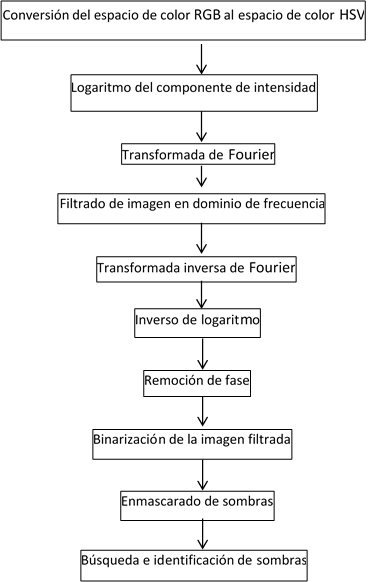
\includegraphics[width=0.5\textwidth]{Imagenes/Homomorfico/flowchart.png}
     \hfill
     \caption{Diagrama de flujo del procesamiento homomórfico}
    \label{flowchart_homomorfico}
\end{figure}

donde $D_0$ es la frecuencia de corte, $c$ controla la forma y pendiente del filtro en la región de transición entre $\gamma_L$ y $\gamma_H$. $D(u,v)$ es la distancia al origen del plano de frecuencias.

Las imágenes a ser analizadas son imágenes satelitales obtenidas desde el sitio web Bing \color{red}\textbf{(poner en referencia de la dirección web del maps)}\color{black}. Se seleccionaron imágenes de diferentes sitios de la Provincia de Misiones, correspondientes a selvas en parques y reservas, en los que se supone mayor presencia de especies de árboles de interés para el presente trabajo. 
En un primer paso se realizó la conversión de la imagen de color rojo, verde y azul (RGB) a la representación matiz, saturación e intensidad (HSI), trabajando sobre la componente de intensidad. La componente de intensidad se obtiene sumando los tres canales rojo, verde y azul y dividiendo por tres (ecuación \ref{RGB-HSI}). 
%%%%%%%%%%%%%%%%%%%%%%%%%%%%%%%%%%%%%% ECUACIÓN %%%%%%%%%%%%%%%%%%%%%%%%%%%%%%%%%%%%%%%%%%%%%%%%%%%%%%%%%
\\
\begin{equation}
	I=\frac{R+G+B}{3},\label{RGB-HSI}
\end{equation}
\\
donde $I$ es el valor de intensidad, $R$, $G$ y $B$ son los valores respectivos de las bandas roja, verde y azul.
%%%%%%%%%%%%%%%%%%%%%%%%%%%%%%%%%%%%%%%%%%%%%%%%%%%%%%%%%%%%%%%%%%%%%%%%%%%%%%%%%%%%%%%%%%%%%%%%%%%%%%%%%  
En un paso siguiente se aplicó el logaritmo a la componente de intensidad de la imagen y seguidamente se obtuvo la transformada de Fourier de la misma, para poder procesar con el filtro de sombras, expresado en la ecuación \ref{filtro homomorfico}. Se multiplicó la matriz de la imagen por la matriz que representa al filtro y luego, al resultado se le aplicó la transformada inversa de Fourier, la función inversa de logaritmo y la remoción de fase, tomando el módulo del número complejo, todo en orden sucesivo. 
%Posteriormente se binarizó la imagen filtrada fijando el valor de umbral en 0,75 en una escala en la que el valor 1 es blanco y 0 es negro, de modo que a los píxeles con valor de intensidad menor al umbral se les asignó el valor cero, y a los que superaban el valor umbral se les asignaba el valor 1. La imagen de salida del filtro de sombras constituye así una máscara que presenta a las sombras resaltadas con píxeles de intensidad blancos. 
Luego se efectuó la selección de las sombras binarizadas mediante técnicas de lógica difusa, en dos etapas. En la primera implementando un inferenciador Sugeno, mediante el cual se discriminaban los píxeles de determinada intensidad , con lo que se descartaron las sombras que no revisten interés para el posterior conteo, es decir aquellas muy pequeñas o muy grandes, estableciendo una ventana de enmascaramiento, que a los efectos prácticos es cuadrada y el criterio de clasificación es de 45\% de píxeles blancos. Una vez completas la binarización y la selección de sombras de interés, se realizó el conteo de las mismas. El diagrama de flujo de la figura \ref{flowchart_homomorfico}  describe las etapas del proceso completo. 


%\color{cyan} %color de texto con 70-80 % o más de avance
\subsection{Procesamiento morfológico (Pasantía)} \label{Morfo}
%revisar definiciones que pueden ir en el marco teórico y aquellas que se definen aquí
Secuencia de actividades para el tratamiento de las imágenes\\
1. Preprocesamiento\\
2. Eliminación de áreas sin sombra\\
3. Primera identificación de objetos oscuros\\
4. Relleno de sombras en copas\\
5. Identificación y relleno de huecos en grandes copas\\
6. Segunda identificación de objetos oscuros\\
7. Búsqueda de pequeños huecos en grandes copas\\
8. Homogeneización de escala de grises en grandes árboles\\
9. Extracción de copas de segmentación\\
10.  Delineación de copas individuales\\

\subsubsection{Preprocesamiento y eliminación de áreas sin sombra}
La imagen es presentada en el formato de escala de grises (formato HSL, de Hue-color, Saturation-saturación, Luminosity-luminosidad) y recortada en el área de interés (las que contienen sombras)
\subsubsection{Primera identificación de objetos oscuros}
Una primera identificación de objetos oscuros se logra a partir de definir a los píxeles de la imagen que tienen un valor menor que la media en la distribución de grises.
\subsubsection{Relleno de sombras en copas}
Este paso es para "suavizar" la textura de las copas de los árboles, rellenando los espacios de sombras.
Si se invierte los valores de los píxeles de la imagen y se le suma el máximo valor de la escala de grises, se obtiene un equivalente a una imagen negativa. Luego se aplica un filtro Rolling Ball con radio de tres píxeles. La imagen resultante se vuelve a invertir.
\subsubsection{Identificación y relleno de huecos en grandes copas}
Según la resolución espacial de la imagen utilizada, una copa de árbol de 7,5 m de diámetro abarca 15 píxeles. Se lleva a cabo una transformación top hat, con un elemento estructurante circular de diámetro de 15 píxeles. Se obtiene entonces una máscara binaria que contiene solamente copas grandes (mayores a 7,5 metros de diámetro).
\subsubsection{ Segunda identificación de objetos oscuros}
Se asume que la mayoría de los píxeles oscuros dentro de las copas de los árboles fueron removidos. Se realiza entonces una segunda identificación de píxeles oscuros, definidos como aquellos menores al 99º percentil de distribuciones en huecos.
\subsubsection{Búsqueda de pequeños huecos en grandes copas}
En las copas grandes existen áreas de huecos o sombras que a los efectos de facilitar la tarea de conteo de copas, es conveniente rellenarlos. Para realizarlo se analiza en una ventana de 7 por 7 píxeles la ocurrencia de valores distintos de cero alrededor de cada píxel. Estos tienen una distribución bimodal, donde los huecos en las copas son aquellos cuyos valores están por encima del 75º percentil. Al finalizar la etapa se identifican tres clases de píxel: los que corresponden a sombras entre árboles, los no sombreados en copas y los que son sombras en las copas. Se constituye una máscara binaria asignando 0 para píxeles fuera de copas y 1 para píxeles dentro de copas.
\subsubsection{Homogeneización de escala de grises en grandes árboles}
Los píxeles de las copas grandes son rellenados con la media de los cuatro mayores valores en una ventana de 7 por 7 píxeles.
\subsubsection{Extracción de copas de segmentación}
Mediante un filtro top bottom se efectua la extracción de copas de diámetro mayor a 3 m, usando un elemento estructural de 6 por 6 píxeles. Luego se umbraliza la imagen con el valor del 0,001 percentil.
\subsubsection{Delineación de copas individuales}
En esta etapa se calcula la distancia entre valores cero y distinto de cero, es decir la distancia del píxel al borde de la copa. Por medio de una ventana cuadrada se calcula el máximo local, y se genera una dilatación que duplique el diámetro.





\color{cyan} %color de texto con 70-80 % o más de avance
\subsection{Invariante de color (paper RSASE)} \label{Metodología}
\subsubsection{Metodología propuesta IIC}
En esta sección se describen los pasos del método de procesamiento necesarios para obtener la máscara automática de sombras de la imagen aérea. La figura \ref{diagrama_procesamiento} representa la secuencia de procesamiento.

\begin{figure}
    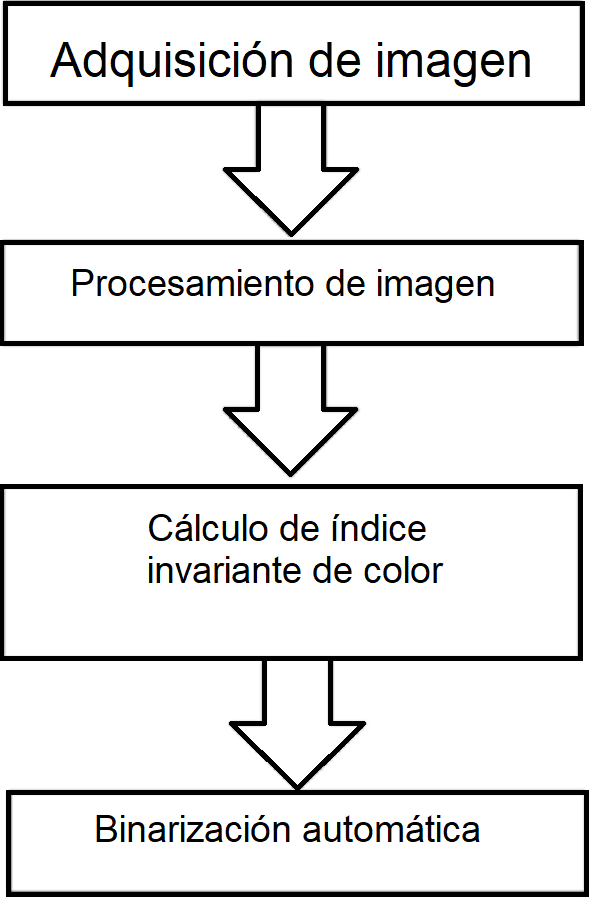
\includegraphics[width=\textwidth]{Imagenes/flowchart.png}
     \hfill
     \caption{Diagrama del procesamiento}
    \label{diagrama_procesamiento}
\end{figure}

\paragraph{Adquisición de la imagen}
El punto de partida de la metodología propuesta es la captura de imágenes aéreas. Entre los pocos requerimientos en esta etapa se destaca que las condiciones de luz solar deben ser las apropiadas para generar proyecciones de sombra. Aquí se consideran imagenes representativas de un área de selva nativa en la provincia de Misiones, Argentina, que han sido capturadas mediante VANT sobrevolando porciones de selva en parques y reservas naturales, en las cuales habría presencia de ejemplares de árboles de interés. Para garantizar una mejor captura de imágenes con sombra, se seleccionó un intervalo de tiempo que abarca desde las 3 p.m. hasta las 4 p.m., que es cuando la posición relativa del sol facilita la proyección de sombras sobre el dosel. Las imágenes fueron capturadas durante el invierno meridional, específicamente en el mes de agosto, cuando las sombras proyectadas son mayores para ese horario. Se usó un VANT modelo Mini 2 del fabricante DJI, equipado con una cámara con resolución de 12 Megapíxeles. La altura de vuelo sobre el terreno fue de 50 metros, y el modo en que estuvo configurada la cámara era automático. Las imágens capturadas están en formato JPG con una resolución de 4000 x 2250 píxeles, con una resolución espacial de 3 cm/pixel aproximadamente. Para ejecutar el algoritmo se usó una computadora laptop común con un procesador Intel Core i5. En cuanto a los scripts, están basados en códigos de Octave. Se analizó un total de 19 imágenes.

\paragraph{Preprocesamiento de imagen} 
Para facilitar el procesamiento y posterior análisis, las imágenes de los diferentes sitios deben ser recortadas par anormalizar el tamaó y ser filtradas para estandarizar algunos atributos.
\paragraph{Cálculo de índice invariante de color}
Con base en imágenes filtradas RGB, el invariante de color $\Psi$ se calcula por medio de la ecuación \ref{invariante de color}
 %%%%%%%%%%%%%%%%%%%%%%%%%%%%%%%%%%%%%% ECUACIÓN %%%%%%%%%%%%%%%%%%%%%%%%%%%%%%%%%%%%%%%%%%%%%%%%%%%%%%%%%
\\
\begin{equation}
	\Psi=\frac{4}{\pi} arctan\left(\frac{B\textsubscript{1}-B\textsubscript{2}}{B\textsubscript{1}+B\textsubscript{2}}\right),\label{invariante de color}
\end{equation}
\\
%%%%%%%%%%%%%%%%%%%%%%%%%%%%%%%%%%%%%%%%%%%%%%%%%%%%%%%%%%%%%%%%%%%%%%%%%%%%%%%%%%%%%%%%%%%%%%%%%%%%%%%%%
 donde $B_1$ y $B_2$ son dos bandas diferentes de color, rojo, verde o azul. El índice invariante de color $\Psi$ toma un valor entre -1 y 1. Si se aplica la ecuación a las bandas correspondientes $B_1$ y $B_2$, el resultado es una matriz de idéntico tamaño al de la imagen, en la que cada píxel contiene el valor del índice invariante de color. Según sea la combinación entre bandas, hay hasta seis posibilidades, siendo una mitad complementaria de la otra mitad. Por esta razón sólo se tienen en cuenta tres de esas posibilidades. La matriz de índice invariante de color se usó para analizar las partes sombreadas y no sombreadas de la imagen. Así, para las tres combinaciones a implementar, se describen en las ecuaciones \ref{psibr}, \ref{psibg} y \ref{psigr}:
 \\
 \\
\begin{equation}
	\Psi_{BR}=\frac{4}{\pi} arctan\left(\frac{B\textsubscript{B}-B\textsubscript{R}}{B\textsubscript{B}+B\textsubscript{R}}\right),\label{psibr}
\end{equation}
\\
\\
\begin{equation}
	\Psi_{BG}=\frac{4}{\pi} arctan\left(\frac{B\textsubscript{B}-B\textsubscript{G}}{B\textsubscript{B}+B\textsubscript{G}}\right),\label{psibg}
\end{equation}
\\
\\
\begin{equation}
	\Psi_{GR}=\frac{4}{\pi} arctan\left(\frac{B\textsubscript{G}-B\textsubscript{R}}{B\textsubscript{G}+B\textsubscript{R}}\right),\label{psigr}
\end{equation}
\\
donde $B_{B}$, $B_{G}$, y $B_{R}$ son los canales azul, verde y rojo respectivamente.
\paragraph{Binarización automática}
 La binarización permite separar la imagen en dos regiones, con sombra y sin sombra, mediante la matriz de índice invariante de color y un valor de umbral, calculado como la frecuencia acumulada de la distribución de valores individuales de IIC. Esta máscara que se obtiene, denominada máscara automática, se compone de píxeles de valores 1 y 0, correspondiendo el valor de 1 al de las regiones sombreadas de la imagen. En la composición de la máscara binaria se asume un valor de 1 (visualizado en blanco) para las regiones sombreadas. Tomando la distribución de frecuencia acumulada del índice invariante de color, se determina el valor umbral que excede los percentiles 60º, 70º, 80º, 85º, 90º y 95º. De este modo, en el presente trabajo, se obtienen seis máscaras, cada una correspondiente al valor de umbral de cada percentil. Luego el valor de umbral es variable y es calculado para cada imagen para un percentil determinado. La calidad de cada máscara automática obtenida es evaluada al compararse con una máscara manual obtenida por un experto humano para la correspondiente imagen.

\paragraph{Comparación cuantitativa con un índice de calidad}
Para establecer un índice de calidad (QI) del desempeño de la selección automática, se proponen tres índices: el primero ($QI_1$) se obtiene del cociente entre la suma de todos los píxeles de la matriz binaria, obtenida como consecuencia de la intersección de la máscara manual y la máscara automática, y la suma de todos los elementos de la máscara manual (\ref{qi1}). El segundo índice ($QI_2$) se obtiene dividiendo la suma de elementos de la intersección por la suma de los elementos de la máscara automática (\ref{qi2}); y el tercer índice ($QI_3$) se obtiene dividiendo la suma de los elementos de la intersección por la suma de los elementos de la unión de la máscara manual y automática (\ref{qi3}.
\\
\\
 \begin{equation}
    QI_1=\frac{\Sigma _{i,j}(M_M\cap M_A )}{\Sigma _{i,j}(M_M ) }
    \label{qi1}
\end{equation}
\\
\\
 \begin{equation}
    QI_2=\frac{\Sigma _{i,j}(M_M\cap M_A )}{\Sigma _{i,j}(M_A ) }
    \label{qi2}
\end{equation}
\\
\\
\begin{equation}
    QI_3=\frac{\Sigma _{i,j}(M_M\cap M_A )}{\Sigma _{i,j}(M_M \cup M_A ) }
    \label{qi3}
\end{equation}
\\
\\
Donde $M_M$ es la máscara binaria manual y $M_A$ es la máscara binaria automática. Cada uno de los índices precedentes toma valores de 0 a 1, siendo 0 el caso en que no hay ninguna coincidencia entre máscaras, y 1 indica plena coincidencia. Para los tres índices, el numerador es la intersección entre ambas máscaras, manual y automática, ya que es un buen indicador de coincidencia entre ambas. El denominador en tanto da un valor de referencia que parametriza el índice. La intersección y la unión son operaciones lógicas que se aplican a cada píxel, de modo que es una condición necesaria que sendas máscaras binarias automática y manual que serán comparadas entre sí, sean del mismo tamaño y de áreas de captura coincidentes. En un nivel de píxel, la intersección es una operación lógica "and", por lo que, al ser cero uno de sendos píxeles comparados, el resultado de la operación dará cero. Por otro lado, la unión implica una operación a nivel de píxel de tipo "or", y siendo uno de sendos píxeles de valor uno, el resultado será uno. El objetivo de este índice es evaluar cuanto se asemeja la selección automática del algoritmo a la selección manual. Así, el mayor valor que corresponde a 1 implica una selección automática exacta, mientras que valores más bajos cercanos a cero corresponden a una pobre correlación entre sendas selecciones.


\paragraph{Etapa de filtrado}
Para quitar el ruido de la imagen, se implementa un filtro de mediana. Para evaluar cómo la etapa de filtrado afecta el desempeño de la selección automática, se realizaron para cada imagen tres pruebas con diferentes configuraciones de filtro, con vecindad de tres por tres, seis por seis, y  doce por doce pixeles. Para cada caso se propuso un conjunto de tres índices de calidad, descriptos en las ecuaciones \ref{qi5}, \ref{qi6} y \ref{qi7}
\\
\\
 \begin{equation}
    QI_5=\frac{\Sigma _{i,j}(M_{NF}\cap M_{WF})}{\Sigma _{i,j}(M_{NF}) }
    \label{qi5}
\end{equation}
\\
\\
 \begin{equation}
    QI_6=\frac{\Sigma_{i,j}(M_{NF}\cap M_{WF})}{\Sigma _{i,j}(M_{WF}) }
    \label{qi6}
\end{equation}
\\
\\
\begin{equation}
    QI_7=\frac{\Sigma _{i,j}(M_{NF}\cap M_{WF})}{\Sigma _{i,j}(M_{NF}\cup M_{WF}) }
    \label{qi7}
\end{equation}
\\
\\
en donde $M_{NF}$ es la máscara binaria automática obtenida sin filtrado, y $M_{WF}$ es la obtenida luego de la etapa de filtrado.



\color{black} 
%\subsection{Machine learning (¿?)}




%Las Tesis  en el marco de la Carrera del Doctorado en Ciencias Aplicadas (DCA) deberán ser escritas en idioma Español, utilizando letra tipo Arial, tamaño 11 puntos, y formato de hojas tipo A4, numeradas en el margen inferior derecho, con interlineado 1,5; sin separación automática de sílabas al fin de línea y con los cuatro márgenes de 2,5 cm.

%El contenido de las Tesis deberá incluir los siguientes ítems y en el siguiente orden:\newline
%●	Carátula (con el formato solicitado por el DCA que se adjunta al presente Anexo)\newline
%●	Agradecimientos\newline
%●	Índice\newline
%●	Listado de Abreviaturas (en caso de que lo considere conveniente)\newline
%●	Resumen en Español\newline
%●	Palabras Claves en Español (tres a seis palabras claves separadas por comas. La primera letra de cada palabra clave debe empezar con mayúscula)\newline
%●	Resumen en Inglés (Abstract)\newline
%●	Palabras Claves en Inglés (tres a seis palabras claves separadas por comas. La primera letra de cada palabra clave debe empezar con mayúscula)\newline
%●	Capítulo 1: Introducción (deberá contener el planteo del problema a resolver, los objetivos generales y específicos y una breve explicación de lo que versará la Tesis)\newline
%●	Capítulo 2: Marco Teórico\newline
%●	Capítulo 3: Metodología\newline
%●	Capítulo 4: Resultados y Discusión (O bien, se podrá presentar en dos Capítulos separados: Capítulo 4: Resultados y Capítulo 5: Discusión)\newline
%●	Capítulo 5: Conclusiones (Deben presentarse en párrafos cortos y concretos. No deben hacer referencia a trabajos futuros ni a hipótesis no incluidas en el trabajo).\newline
%●	Recomendaciones para Trabajos Futuros\newline
%●	Producción Científica (surgida del trabajo de Tesis)\newline
%✔	Publicaciones en Revistas y Capítulos de Libros\newline
%✔	Presentaciones a Congresos\newline
%●	Proyecto/s de Investigación dentro del/los cual/es se desarrolló la Tesis (si hubiera/n)\newline
%●	Beca/s y Subsidio/s con los que se financió la Tesis (si hubieran)\newline
%●	Apéndices o Anexos (se reservan para detallar técnicas originales utilizadas o análisis teóricos que impedirían seguir fluidamente el trabajo si se incluyeran en el texto). Las tablas y figuras de los apéndices o anexos deben comenzar otra numeración diferente a la de los capítulos.\newline

%Aclaraciones

%⮚	El listado de Referencias bibliográficas se podrá incorporar al final de cada capítulo, ó todas juntas al final de la Tesis, las mismas serán listadas en el orden en que aparecen citadas en el texto. \newline
%Formato de las Referencias\newline
%Estilo de las Referencias\newline
%En el texto de la Tesis: indique las referencias por número (s) entre corchetes en línea con el texto. Cuando se menciona a los autores, siempre se deben proporcionar los números de referencia.
%Ejemplo: '..... como se demostró [3,6]. Barnaby y Jones [8] obtuvieron un resultado diferente ... '
%Lista de Referencias\newline
%Numere las referencias (números entre corchetes) en la lista en el orden en que aparecen en el texto, como se indica a continuación:5
%\paragraph{Referencia a una publicación de revista}
%[1] J. van der Geer, J.A.J. Hanraads, R.A. Lupton, The art of writing a scientific article, J. Sci. Commun. 163 (2010) 51–59.https://doi.org/10.1016/j.Sc.2010.00372.
%\paragraph{Referencia a una publicación de revista con un número de artículo}
%[2] J. van der Geer, J.A.J. Hanraads, R.A. Lupton, 2018. The art of writing a scientific article.Heliyon. 19, e00205.https://doi.org/10.1016/j.heliyon.2018.e00205.
%\paragraph{Referencia a un libro}
%[3] W. Strunk Jr., E.B. White, The Elements of Style, fourth ed., Longman, New York, 2000.
%\paragraph{Referencia a un capítulo en un libro editado}
%[4] G.R. Mettam, L.B. Adams, How to prepare an electronic version of your article, in: B.S. Jones, R.Z. Smith (Eds.), Introduction to the Electronic Age, E-Publishing Inc., New York, 2009, pp. 281–304.
%\paragraph{Referencia a un sitio} web
%[5] Cancer Research UK, Cancer statistics reports for the UK. http://www.cancerresearchuk.org/ aboutcancer/statistics/cancerstatsreport/, 2003 (accessed 13 March 2003).
%\paragraph{Referencia a un conjunto de datos: [conjunto de datos]}
%[6] M. Oguro, S. Imahiro, S. Saito, T. Nakashizuka, Mortality data for Japanese oak wilt disease and surrounding forest compositions, Mendeley Data, v1, 2015. https://doi.org/10.17632/ xwj98nb39r.1
%⮚	Las figuras (gráficos, cuadros, fotografías, otros) deberán numerarse correlativamente en el orden de aparición en el texto y deberán incluir un breve título explicativo en la parte inferior de la figura. Las imágenes y fotografías se designarán como figuras.\newline
%%%%%%%%%%%%%%%%%%%%%%%%%%%%%%%%%%%%%%% FIGURA %%%%%%%%%%%%%%%%%%%%%%%%%%%%%%%%%%%%%%%%%%%%%%%%%%%%%%%%%
%\begin{figure}[ht!]
%    \centering
%    \captionsetup{justification=centering}
%    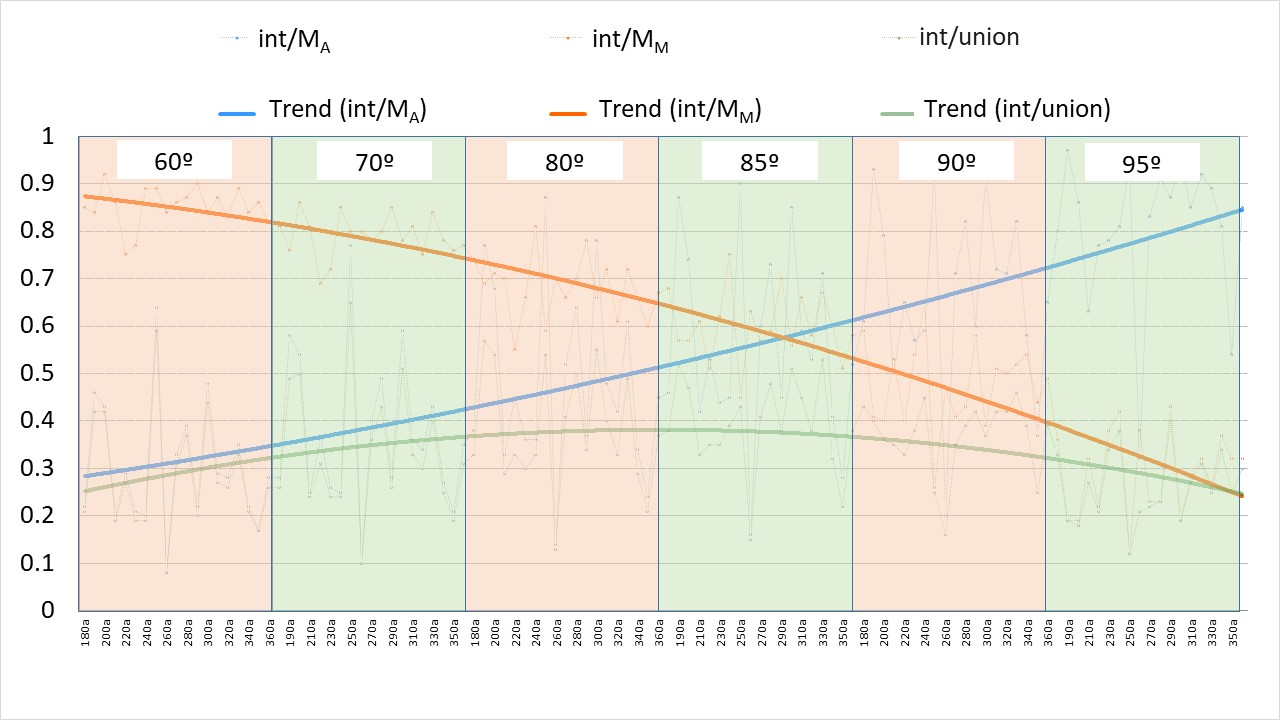
\includegraphics[width=8cm]{grafico.jpg}
%    \caption{Quality Index as a function of the percentile, for the different forest image used. QI\textsubscript{1} in orange, QI\textsubscript{2} in blue and QI\textsubscript{3} in green. The invariant color index used is ψ\textsubscript{BR}}	
 %   \label{qi}
%\end{figure}
%%%%%%%%%%%%%%%%%%%%%%%%%%%%%%%%%%%%%%%%%%%%%%%%%%%%%%%%%%%%%%%%%%%%%%%%%%%%%%%%%%%%%%%%%%%%%%%%%%%%%%%%%
%⮚	Las tablas deberán numerarse correlativamente según su orden de aparición en el texto y en forma independiente de las figuras. Deberán incluir un título explicativo en su parte superior. De ser necesario se agregarán al pie notas explicativas para detallar abreviaturas, signos, medidas, otros, de tal manera que el lector pueda comprender su contenido sin recurrir al texto.
%%%%%%%%%%%%%%%%%%%%%%%%%%%%%%%%%%%%%%%%% TABLA %%%%%%%%%%%%%%%%%%%%%%%%%%%%%%%%%%%%%%%%%%%%%%%%%%%%%%%%%
%\begin{table}[H]
  %  \centering
   % \caption{Evaluation of the superposition of both masks. the manual and the automatic. carried on by the group of experts}
    %\begin{tabular}{|c|c|c|c|c|c|c|c|}
     %  \hline
      %  COLOR INVARIANT INDEX & \multicolumn{6}{ |c|}{\textpsi \textsubscript{BR}}\\%\multicolumn{6}{ }{ |c|} \\
       % \hline
        %PERCENTILE & 60 & 70 & 80 & 85 & 90 & 95\\
        %\hline
        %GOOD & 0.0 & 0.0 & 4.5 & 15.8 & 20.5 & 0.0\\
        %\hline
        %REGULAR & 0.0 & 4.5 & 27.3 & 21.1 & 54.5 & 57.9\\
        %\hline
        %BAD & 100.0 & 95.5 & 68.2 & 63.2 & 25.0 & 42.1\\
        %\hline
        %COLOR INVARIANT INDEX & \multicolumn{6}{ |c|}{\textpsi \textsubscript{BG}}\\
        %\hline
        %PERCENTILE & 60 & 70 & 80 & 85 & 90 & 95\\
        %\hline
        %GOOD & 0.0 & 0.0 & 0.0 & 5.3 & 5.3 & 5.3\\
        %\hline
        %REGULAR & 0.0 & 5.3 & 10.5 & 15.8 & 42.1 & 21.1\\
        %\hline
        %BAD & 100.0 & 94.7 & 89.5 & 78.9 & 52.6 & 73.7\\
        %\hline
        %COLOR INVARIANT INDEX & \multicolumn{6}{|c|}{ \textpsi \textsubscript{GR}}\\
        %\hline
        %PERCENTILE & 60 & 70 & 80 & 85 & 90 & 95\\
        %\hline
        %GOOD & 0.0 & 0.0 & 0.0 & 0.0 & 0.0 & 0.0\\
        %\hline
        %REGULAR & 0.0 & 0.0 & 0.0 & 0.0 & 15.8 & 15.8\\
        %\hline
        %BAD & 100.0 & 100.0 & 100.0 & 100.0 & 84.2 & 84.2\\
        %\hline
    %\end{tabular}
    %\\
    %\raggedleft
    %\label{tablita}
%\end{table}
%%%%%%%%%%%%%%%%%%%%%%%%%%%%%%%%%%%%%%%%%%%%%%%%%%%%%%%%%%%%%%%%%%%%%%%%%%%%%%%%%%%%%%%%%%%%%%%%%%%%%%%%%
%⮚	Las fórmulas y expresiones matemáticas deberán ser escritas dejando dos espacios sobre, debajo y entre cada una de ellas.
%%%%%%%%%%%%%%%%%%%%%%%%%%%%%%%%%%%%%% ECUACIÓN %%%%%%%%%%%%%%%%%%%%%%%%%%%%%%%%%%%%%%%%%%%%%%%%%%%%%%%%%
%\begin{equation}
%	\psi=\frac{4}{\pi} arctan\left(\frac{B\textsubscript{1}-B\textsubscript{2}}{B\textsubscript{1}+B\textsubscript{2}}\right),\label{eq1}
%\end{equation}
%%%%%%%%%%%%%%%%%%%%%%%%%%%%%%%%%%%%%%%%%%%%%%%%%%%%%%%%%%%%%%%%%%%%%%%%%%%%%%%%%%%%%%%%%%%%%%%%%%%%%%%%%
%Las fórmulas se ajustarán al margen izquierdo y serán numeradas correlativamente y entre paréntesis sobre el margen derecho. Debe quedar definido el significado y las unidades utilizadas en cada término de las expresiones.

%⮚	Unidades: debe utilizarse el sistema internacional de unidades (SI).
